\section{Transfer between halos}

Looking at particle-level metrics can be informative, but the majority of
analysis performed on cosmological simulations occurs on bound structures for
good reason; they are what can be accurately observed and easily identified.
The below analysis considers transfer of baryonic material between halos and
their associated lagrangian regions in the initial conditions of the
simulation.

\subsection{Defining halos}

Halos in the following discussion are defined by using the \velociraptor{} structure
finder \citep{}. This structure finder uses a 6D friends-of-friends (FOF) algorithm
with an adaptive linking length for each halo to disentangle mergers. A standard
linking length of $\ell = 0.1$ is used for the initial 3D FOF search for field halos.
The parameter files that were used to find the halos can be found on our \github{}
page here\footnote{\url{https://github.com/jborrow/simba-velociraptor-tools} using
revision {\tt GIT REVISION}} and used the revision {\tt GIT REVISION} of
\velociraptor{}. As the analysis presented here uses halo-level metrics, no galaxy
finder was used, and \velociraptor{} was not ran in galaxy-finding mode.

\subsection{Defining lagrangian regions}

Many methods exist for defining lagrangian regions, but these are mostly used for
zoom-in simulations and some, for example using a cube of particles around a given
halo, could be seen as being non-lagrangian and over-conservative. In the below
discussion the lagrangian regions are defined in the initial conditions in the
following way:
\begin{enumerate}
	\item Find all halos at $z=0$.

    \item For each halo, ID match the particles contained within it with those
		  in the initial conditions. This defines the initial lagrangian region
		  based on the dark matter.

	\item In some cases, discussed below, fill in the holes in this lagrangian
	      region by using a nearest-neighbour search.

	\item For every gas particle in the initial conditions, find the nearest dark
	      matter neighbour. This gas particle is assigned to the same lagrangian
	      region as that dark matter particle.
\end{enumerate}
This allows the definition of the lagrangian region to also extend to the gas
that should be gravitationally bound by that halo at $z=0$.

\subsection{Calculating transfer between lagrangian regions}

Now that the lagrangian regions have been defined, it is possible to consider on
a particle-by-particle basis where particles started and where they ended up.
The algorithm is as follows:
\begin{enumerate}
	\item ID match all particles between the initial and final conditions, including
	      star particles (these are matched to their gas progenitor). Black holes
	      are ignored in this analysis.

	\item Every particle in the $z=0$ final conditions has several possible final
	      states and origins:
	      \begin{itemize}
	            \item Particle resides in a halo $i$
	            \begin{itemize}
	           		\item Particle originated in the same lagrangian region $i$
	           		\item Particle originated in some other lagrangian region $j \neq i$
	           		\item Particle originated outside any lagrangian region $j = -1$
	            \end{itemize}
	            \item Particle resides outside a halo ($i = -1$)
	            \begin{itemize}
	            	\item Particle has never been in any lagrangian region or halo
	            	\item Particle originated in a lagrangian region $j$ and was moved out
	            \end{itemize}
	      \end{itemize}
	      
	\item For every halo and lagrangian region the mass originating from each
	      of the above compopnents is computed and stored.
\end{enumerate}

The source code that performs all of the above analysis is made available by
the authors on \github{}\footnote{\url{https://github.com/jborrow/lagrangian-
transfer}} as a python package.

\subsection{Transfer \emph{into} Halos}

\begin{figure*}
	\centering
	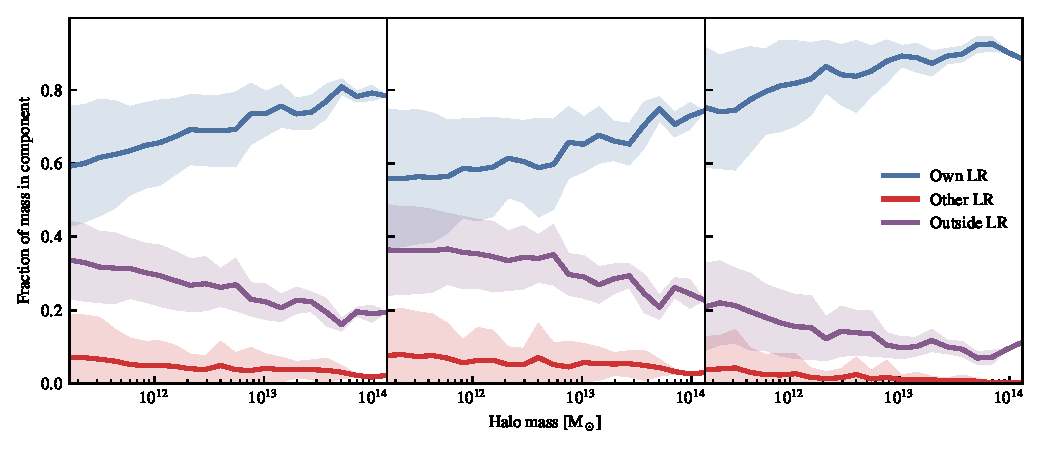
\includegraphics{generated_figures/m50n512s49/component_fraction_mixed.pdf}
	\caption{
		The fraction of baryonic mass originating from each lagrangian component is
		shown as a function of redshift $z=0$ halo mass. {\textit {Left:}} baryonic
		mass, {\textit {center:}} gas mass, and {\textit {right:}} stellar mass. Shaded
		regions show the scatter in a given bin, with one standard deviation of variation
		being shown.
	}
	\label{fig:maintransferresult}
\end{figure*}

The results of this transfer, as a function of halo mass, are shown in Fig.
\ref{fig:maintransferresult}. The general trend is that for an increasing halo mass,
a lagrangian region is able to hold on to more of the original baryonic mass, with
this flattening off around $M_H = 10^{12} \msolar$. For a given halo, sigificantly
more of the gaseous mass originates outside the original lagranigan region as compared
to the stellar mass ($\sim 60 \%$ versus $\sim 90 \%$). The transfer between halos is
at around the $\sim 5-10\%$ baryonic mass level, with this transfer predominantly
originating from the stellar component, as compared to the gaseous component. This comines
nicely with the distnace metrics shown in \S \ref{sec:feedbackmetrics}, which
showed that the dark matter and stars have very similar dynamics.

The transfer between these regions is slightly lower, but is still at the $5-10\%$ level
even for the \nojet{} run. \blue{There really needs to be some disucsion here about
the non-radiative run. These results require such a run to 'blame' the transfer on
feedback rather than simple dynamics}.

%% To Do: we _really_ need that non-radiative run...

In all of the relations there is a high level of scatter. The scatter in these
relations, as with other metrics in astronomy, likely contains more information 
than the relations themselves. A given mass bin contains halos that entertain a range
of 10x in transfer, which is likely dependent on environment. The specific physical
effects that lead to the scatter in these relations will be discussed in a follow-up
paper.

The overall fraction of baryonic mass that is retained by a given lagrangian
region does begin to turn over around $10^{13} \msolar$, however it is unclear
whether this is due to a lack of higher mass halos in the $50 \hmpc$ box. It
is also important to note that the shaded regions in Figure
\ref{fig:maintransferresult} represent the $1\sigma$ scatter in a given bin
and explicitly no \emph{not} include any errors that would occur from a finite
sampling of halos or halo assembly bias.

\subsection{Transfer \emph{out} of Lagrangian Regions}

\begin{figure}
	\centering
	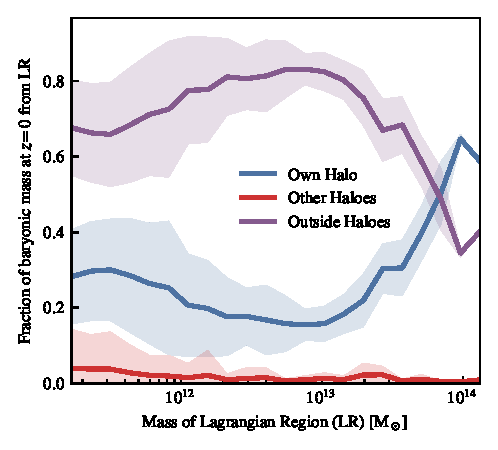
\includegraphics{generated_figures/m50n512s49/inverse_component_fraction.pdf}
	\caption{The fate of gas that begins in lagrangian regions, as a function of
	initial lagrangian region mass. \blue{Should probably
	plot the line for the $z=2$ case here.} }
	\label{fig:transferoutoflrs}
\end{figure}

The clear inverse to the above discussion is to consider what happens to the gaseous
material that originated in a given lagrangian region. Now looking at the results as
a function of lagrangian region mass (this is slightly higher than the eventual
halo mass as the baryon fraction of a given halo is lower than the cosmic mean), it
is clear that there is an even more significant transfer \emph{out} of lagrangian
regions than \emph{into} halos (see Figure \ref{fig:transferoutoflrs}). Only 
approximately $20\%$ of the gas initially resident in a given lagrangian region
makes it into the $z=0$ halo.

The relation between halo mass and transfer out of a given lagrangian region is
relatively flat; this suggests that the origin of the baryon fraction is transfer
prodcued by flows \emph{into} the lagrangian region; i.e. the baryon fraction of
a given galaxy is driven by late-stage cold flows. \blue{This is a bit of a
dubious statement; how can we solidify it? Am I correct?}. Every lagrangian region
begins with the universal baryon fraction, and so with equal fractions of those
baryons ending up in the associated halos, the only way that the baryon fraction
of a given halo can be changed is due to external forces (i.e. accretion from
outside any lagrangian region).

